\documentclass{if-beamer}

% --------------------------------------------------- %
%                  Presentation info	              %
% --------------------------------------------------- %
\title[Projeto -- Etapa 2]{Arquitetura HIL para teste de sistemas embarcados como \textit{vehicle interface} de veículos autônomos baseados no Autoware}
\subtitle{Projeto -- Etapa 2}

\author[G. Toffanetto, J. L. Barraza]{\texorpdfstring
	{Gabriel Toffanetto França da Rocha 
		\\ \vspace{1mm} 
		\small{\href{mailto:g289320@dac.unicamp.br}{g289320@dac.unicamp.br}}
	}
	{Gabriel Toffanetto França da Rocha} \\
	\normalsize \vspace{2mm}
	Juan Luis Barraza Ramirez \\
	\small \vspace{1mm} j272583@dac.unicamp.br
}

\institute[LMA/FEM/Unicamp]{\small{Professor Dr. Rodrigo Moreira Bacurau
  \\ \vspace{2mm}
  IM420X -- Projeto de Sistemas Embarcados de Tempo Real
  \\ \vspace{4mm}
  Faculdade de Engenharia Mecânica
  \\ \vspace{1mm}
  Universidade Estadual de Campinas}
}

\date{22 de outubro de 2024}

\logo{
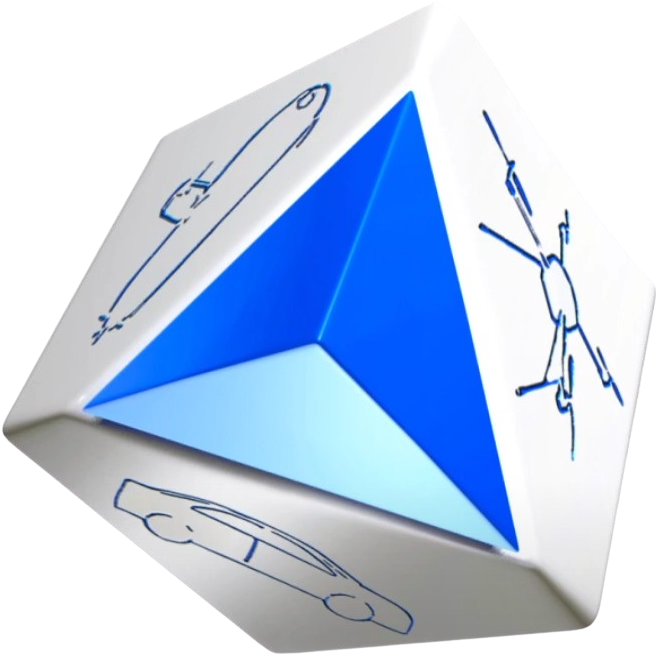
\includegraphics[width=1.2cm]{img/core/Logo_LMA_icon.png}
}


\subject{IM420X - Projeto final: Etapa 2} % metadata

\graphicspath{{img/}}

\setbeamertemplate{caption}[numbered]

\newcolumntype{b}{>{\columncolor{white}}c}


\hypersetup{pdfpagemode=FullScreen}


% --------------------------------------------------- %
%                    Title + Schedule                 %
% --------------------------------------------------- %

\begin{document}

\begin{frame}
  \titlepage
\end{frame}

\begin{frame}{Schedule}
  \tableofcontents
\end{frame}

% --------------------------------------------------- %
%                      Presentation                   %
% --------------------------------------------------- %

\section{Introdução}

\begin{frame}{Proposta}
	
	\begin{columns}
		
		\begin{column}{0.7\textwidth}
			
				\begin{figure}[H]
				\centering
				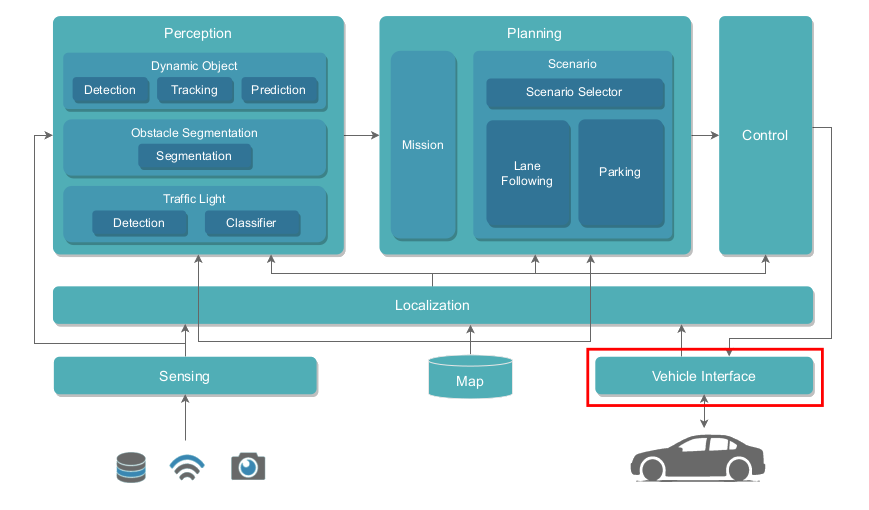
\includegraphics[width=\linewidth]{img/architecture.png}
				\caption{Escopo do projeto na arquitetura Autoware.}
				\label{fig:architecture}
			\end{figure}
			
		\end{column}
		
		\hspace{-0.5cm}
		
		\begin{column}{0.5\textwidth}
			
				\begin{figure}[H]
				\centering
				\includegraphics[width=\linewidth]{img/architecture_HIL}
				\caption{Arquitetura de teste do \textit{hardware}.}
				\label{fig:architecture_HIL}
			\end{figure}
			
		\end{column}
		
	\end{columns}
	
\end{frame}

\section{Estados do sistema}

\begin{frame}{Estados do sistema}
	
	
	\begin{figure}[H]
		\centering
		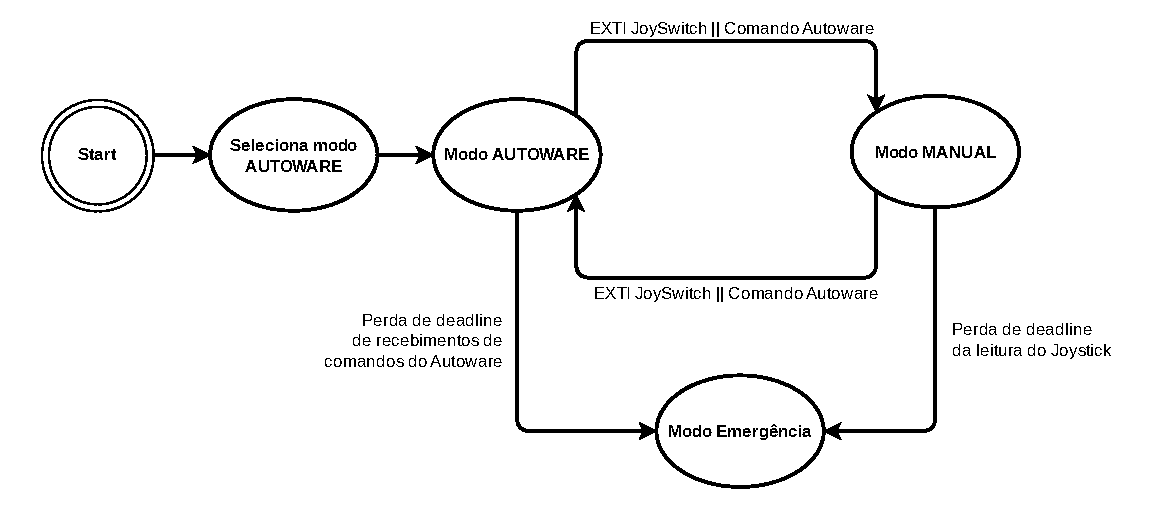
\includegraphics[width=\linewidth]{img/maquinadeestados}
		\caption{Máquina de estados do sistema.}
		\label{fig:maquinadeestados}
	\end{figure}
	
	
\end{frame}


\section{Tarefas}



\begin{frame}{Diagrama do sistema}
	
	% TODO: \usepackage{graphicx} required
	\begin{figure}
		\centering
		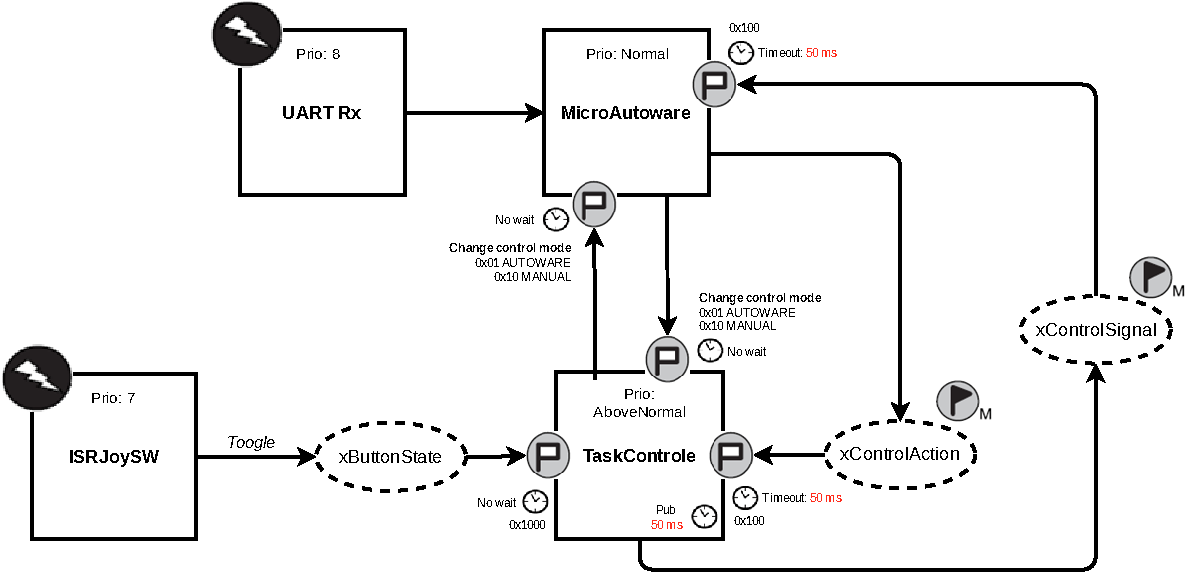
\includegraphics[width=0.95\linewidth]{img/system_diagram}
		\caption{Diagrama do sistema.}
		\label{fig:systemdiagram}
	\end{figure}
	
\end{frame}



\begin{frame}{Descrição das tarefas}
	
\begin{block}{\textbf{Tarefa}}
	
	\centering
	
	\begin{tabular}{c|p{8cm}}
		\textbf{Nome} & TaskControle \\
		\hline
		\textbf{Prioridade}& AboveNormal \\
		\hline
		\textbf{Tamanho da stack} & 500 kB \\
		\hline
		\textbf{Detalhes} & Realiza o controle do veículo utilizando a referência dada pelo \textit{joystick} ou pelo Autoware, dado o modo de operação, podendo ser MANUAL ou AUTOWARE, respectivamente. A alteração do modo é feita por \textit{ThreadFlag}, gerada por ISR ou pelo Autoware. Em caso do modo de operação AUTOWARE, os sinais de controle são recebidos por variável global e sincronizados por \textit{ThreadFlag}, com tempo de X ms, onde caso não receba, entra em algum modo de segurança. Em caso de operação MANUAL,  o \textit{joystick} é lido por DMA, convertendo os valores analógicos em sinais de controle, onde também caso haja algum erro, o modo de emergência é acionado. O sinal de controle é enviado para o carro por meio de uma variável global, que é enviada para o MicroAutoware e sincronizado por \textit{ThreadFlag}. \\
	\end{tabular}
	
\end{block}	
	
\end{frame}



\begin{frame}{Descrição das tarefas}

\begin{block}{\textbf{Tarefa}}
	
	\centering
	
	\begin{tabular}{c|p{8cm}}
		\textbf{Nome} & MicroAutoware \\
		\hline
		\textbf{Prioridade}& Normal \\
		\hline
		\textbf{Tamanho da stack} & 3500 kB \\
		\hline
		\textbf{Detalhes} & Leitura dos \textit{subscribers} Autoware, leitura dos \textit{subscribers} CARLA, envio das informações para a TaskControle, recebimentos das informações da TaskControle, escrita dos \textit{publishes} Autoware, escrita dos \textit{publishers} CARLA. \\
	\end{tabular}
	
\end{block}	

\end{frame}




\begin{frame}{Fluxograma TaskControl}
	
	\begin{figure}[H]
		\centering
		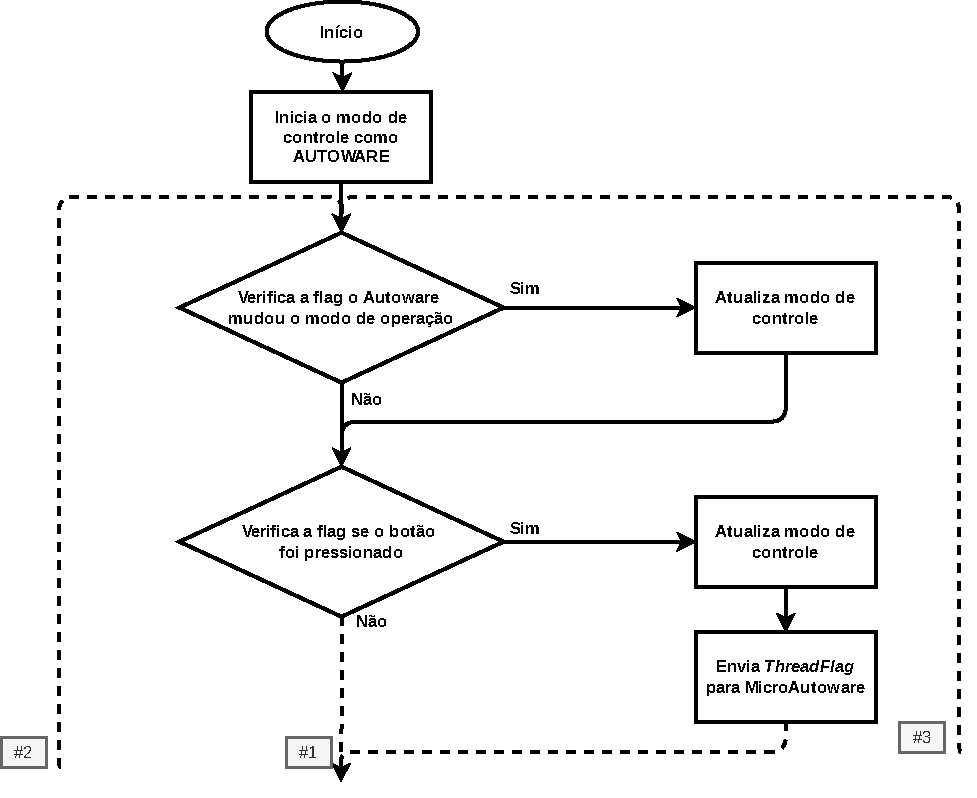
\includegraphics[width=0.6\linewidth]{img/fluxograma_taskcontrol_1}
		\caption{Fluxograma da tarefa TaskControl (Parte 1/2).}
		\label{fig:fluxograma_taskcontrol_1}
	\end{figure}
	
\end{frame}


\begin{frame}{Fluxograma TaskControl}



	\begin{figure}[H]
		\centering
		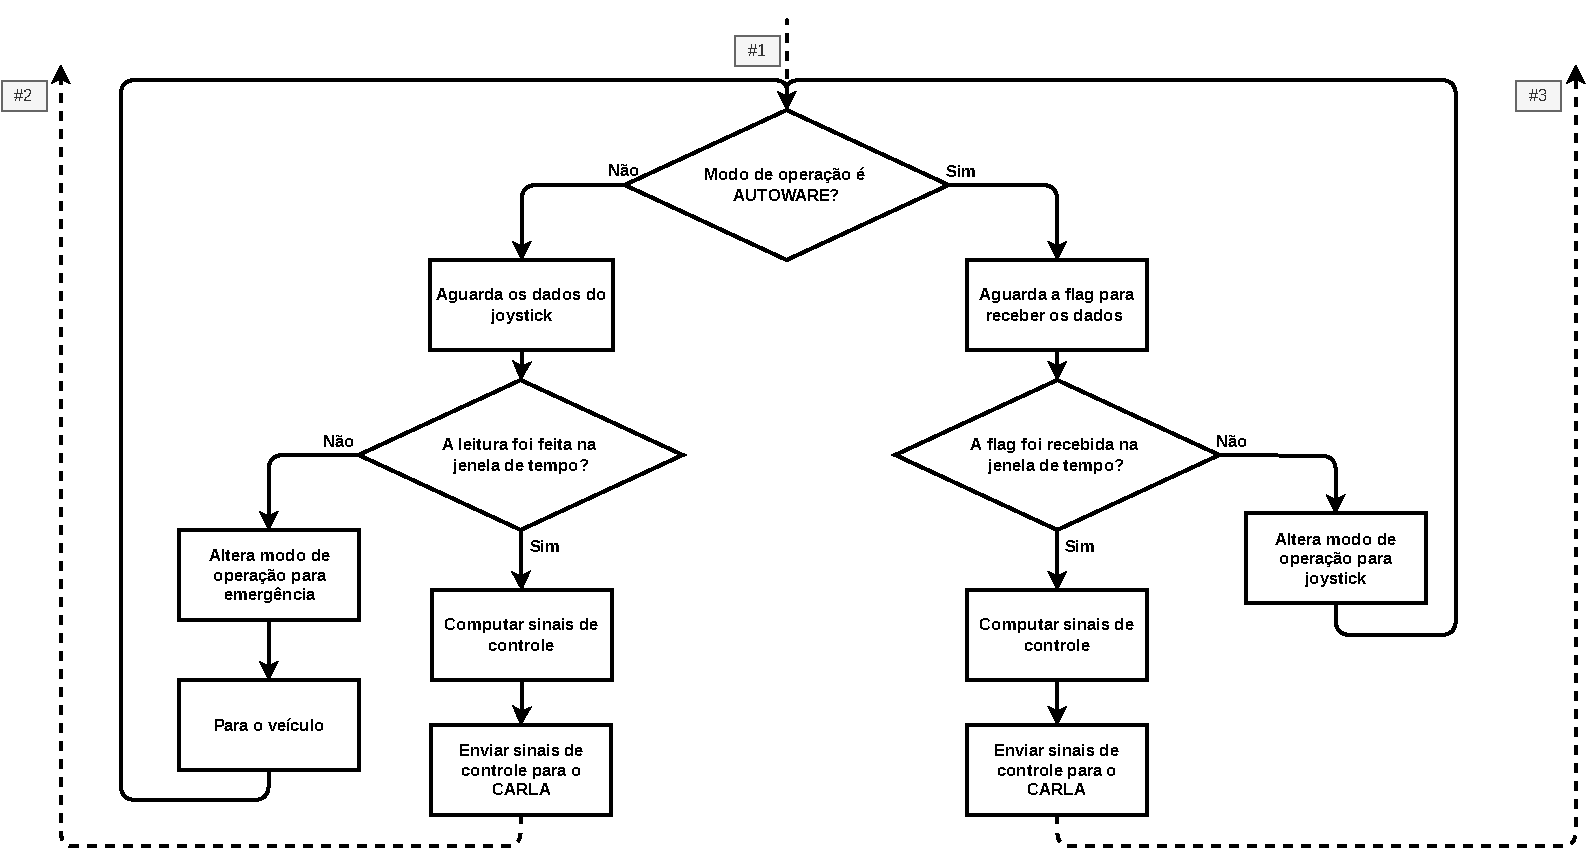
\includegraphics[width=0.8\linewidth]{img/fluxograma_taskcontrol_2}
		\caption{Fluxograma da tarefa TaskControl (Parte 2/2).}
		\label{fig:fluxograma_taskcontrol_2}
\end{figure}

\end{frame}


\begin{frame}{Fluxograma ISR JoySW}



\begin{figure}[H]
	\centering
	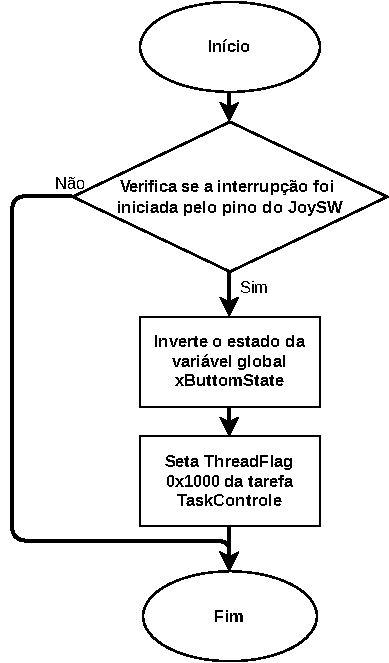
\includegraphics[width=0.29\linewidth]{img/fluxograma_joysw}
	\caption{Fluxograma da ISR JoySW.}
	\label{fig:fluxograma_joysw}
\end{figure}

\end{frame}



\section{Sincronização e comunicação entre tarefas}

\begin{frame}{Sincronização entre tarefas}
	
	\begin{columns}
		
		\begin{column}{0.5\textwidth}
			
				\begin{block}{Sinalização \texttt{xButtonState}}
				
				\begin{itemize}
					\item \textbf{Objeto:} \textit{ThreadFlag}
					\item \textbf{Flag:} 0x1000
					\item \textbf{Modo:} \textit{No wait}
					\item \textbf{Descrição:} Sinaliza ocorrência da interrupção do botão JoySW.
					
				\end{itemize}
				
			\end{block}
	

			\begin{block}{Sinalização \texttt{xControlAction}}
			
			\begin{itemize}
				\item \textbf{Objeto:} \textit{ThreadFlag}
				\item \textbf{Flag:} 0x0100
				\item \textbf{Modo:} \textit{Timeout} XX ms
				\item \textbf{Descrição:} Sinaliza o recebimento de dados pela variável global \texttt{xControlAction}.
				
			\end{itemize}	
			
			\end{block}
			
		\end{column}
		
		\begin{column}{0.5\textwidth}
			
			\begin{block}{Sinalização \texttt{xControlSignal}}
				
				\begin{itemize}
					\item \textbf{Objeto:} \textit{ThreadFlag}
					\item \textbf{Flag:} 0x0100
					\item \textbf{Modo:} \textit{Timeout} XX ms
					\item \textbf{Descrição:} Sinaliza o recebimento de dados pela variável global \texttt{xControlSignal}.
					
				\end{itemize}	
				
			\end{block}
			
		\end{column}
		
	\end{columns}
	
\end{frame}

\begin{frame}{Comunicação entre tarefas}

	\begin{columns}
	
	\begin{column}{0.55\textwidth}
		
		\begin{block}{Alteração do modo de condução por interrupção JoySW}
			
			\begin{itemize}
				\item \textbf{Objeto:} \textit{ThreadFlag}
				\item \textbf{Flags:}
				\begin{itemize}
					\item Modo de controle alterado para AUTOWARE: 0x01
					\item Modo de controle alterado para MANUAL: 0x10
					
				\end{itemize}
				\item \textbf{Modo:} \textit{No wait}
				\item \textbf{Descrição:} Realiza a sincronização do modo de operação da tarefa TaskControle para a MicroAutoware.
				
			\end{itemize}
			
		\end{block}
		
	\end{column}
	
	\begin{column}{0.55\textwidth}
		
		\begin{block}{Alteração do modo de condução pelo Autoware}
			
			\begin{itemize}
				\item \textbf{Objeto:} \textit{ThreadFlag}
				\item \textbf{Flags:}
				\begin{itemize}
					\item Modo de controle alterado para AUTOWARE: 0x01
					\item Modo de controle alterado para MANUAL: 0x10
					
				\end{itemize}
				\item \textbf{Modo:} \textit{No wait}
				\item \textbf{Descrição:} Realiza a sincronização do modo de operação da tarefa MicroAutoware para a TaskControle.
				
			\end{itemize}
			
		\end{block}
		
	\end{column}
	
\end{columns}

\end{frame}

\section{Proteção de recursos}

\begin{frame}{Proteção de recursos}
	
	\begin{columns}
		
		\begin{column}{0.5\textwidth}
			
			\begin{block}{Variável global \texttt{xControlSignal}}
				
				\begin{itemize}
					\item Protegida por MUTEX.
					\begin{itemize}
						\item \texttt{MutexControlSignal}
						
					\end{itemize}
				\end{itemize}
				
			\end{block}
			
		\end{column}
		
		\begin{column}{0.5\textwidth}
			
			
			
			\begin{block}{Variável global \texttt{xControlAction}}
				
				\begin{itemize}
					\item Protegida por MUTEX.
					\begin{itemize}
						\item \texttt{MutexControlAction}
						
					\end{itemize}
					
				\end{itemize}
				
			\end{block}
			
		\end{column}
		
	\end{columns}
	
\end{frame}


\section{Padronização de projeto}

\begin{frame}{Padronização de projeto}
	
	\begin{block}{}
		\centering
		\vspace{1mm}
		Domínio ROS $\times$ Domínio FreeRTOS
		\vspace{1mm}
		
	\end{block}
	
	\begin{columns}
		
		\begin{column}{0.42\textwidth}
			
			\begin{block}{Domínio ROS}
				
				\begin{itemize}
					\item \textit{Vehicle interface};
					\item Padronização de código do ROS.
				\end{itemize}
				
			\end{block}
		
			\begin{block}{Domínio FreeRTOS}
			
				\begin{itemize}
					\item Padronização padrão da disciplina.
				\end{itemize}
			
			\end{block}
			
		\end{column}
		
		\begin{column}{0.45\textwidth}
			
			\begin{block}{Padronização de código ROS}
				
				\begin{itemize}
					\item Subscriber: \texttt{nome\_subscriber\_sub\_}
					\item Publisher: \texttt{nome\_subscriber\_pub\_}
					\item Mensagem: \texttt{nome\_mensagem\_msg\_}
					\item Node: \texttt{nome\_do\_node}
					\item Callback: \texttt{nome\_do\_topico\_callback}
					
				\end{itemize}
				
			\end{block}
			
		\end{column}
		
	\end{columns}

	\vspace{5mm}

	\boxyellow[0.6]{\centering Considera-se que as padronizações não irao se misturar!}
	
\end{frame}


\section{Cronograma}

\begin{frame}{Cronograma}
	
	
\begin{table}
	\centering
	\small{
		\begin{tabular}{|b|b|b|b|b|b|b|b|b|b|}
			\hline
			\textbf{Atividade/Semana} & 1 \cellcolor{lightgray} & \textbf{2} \cellcolor{lightgray} & 3 \cellcolor{lightgray} & \textbf{4} & 5 & 6 & \textbf{7} & 8 & \textbf{9} \\
			\hline
			Proposta do projeto  & \cellcolor{unifeiblue} &  &  &  &  &  &  &  &  \\
			\hline
			Projeto de \textit{hardware} e \textit{software}  &  & \cellcolor{unifeiblue} & \cellcolor{unifeiblue} &  &  &  &  &  &  \\
			\hline
			Integração do STM com o micro-ROS  &  & \cellcolor{unifeiblue} &  &  &  &  &  &  &  \\
			\hline
			Integração do micro-ROS com o Autoware  &  &  & \cellcolor{unifeiblue} & \cellcolor{unifeiblue} & \cellcolor{unifeiblue} &  &  &  &  \\
			\hline
			Implementação das tarefas do sistema embarcado  &  &  &  & \cellcolor{unifeiblue} & \cellcolor{unifeiblue} & \cellcolor{unifeiblue} & \cellcolor{unifeiblue} &  &  \\
			\hline
			Construção do ambiente de testes  &  &  &  &  & \cellcolor{unifeiblue} & \cellcolor{unifeiblue} & \cellcolor{unifeiblue} &  &  \\
			\hline
			Realização dos testes  &  &  &  &  &  &  & \cellcolor{unifeiblue} & \cellcolor{unifeiblue} & \cellcolor{unifeiblue} \\
			\hline
			Escrita do relatório  &   & \cellcolor{unifeiblue} & \cellcolor{unifeiblue} & \cellcolor{unifeiblue} & \cellcolor{unifeiblue} & \cellcolor{unifeiblue} & \cellcolor{unifeiblue} & \cellcolor{unifeiblue} & \cellcolor{unifeiblue} \\
			\hline
		\end{tabular}
	}
	\caption{Cronograma de atividades.}
	\label{tab:crono}
\end{table}
	
	\begin{itemize}
		\small
		\item \textbf{Semana 2:} Apresentação Etapa 1
		\item \textbf{Semana 4:} Apresentação Etapa 2
		\item \textbf{Semana 7:} Apresentação Etapa 3
		\item \textbf{Semana 9:} Apresentação Final
	\end{itemize}
	
\end{frame}


% -------------------------------------------------
%               Bibliografia.
%--------------------------------------------------
\section{Referências bibliográficas}
\begin{frame}{Referências bibliográficas}
   %\bibliographystyle{acm}
   \bibliography{bibliografia.bib}
\end{frame}



\begin{frame}{}
	
	\begin{block}{}
		
		\centering
		\Huge{Obrigado!}
		
		\LARGE
		
		\vspace{5mm}
		
		Dúvidas?
		
	\end{block}
	
	\vspace{4mm}
	
	\begin{figure}[H]
		\centering
		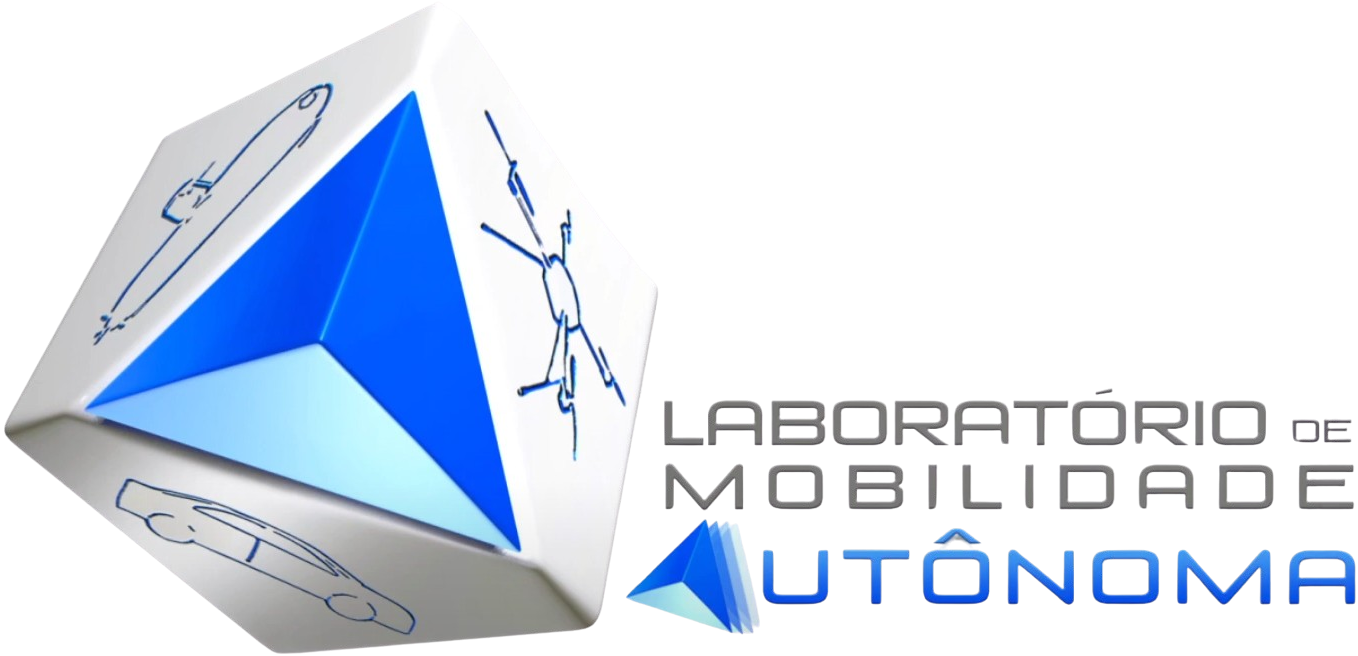
\includegraphics[width=0.5\linewidth]{img/core/Logo_LMA.png}
	\end{figure}
	
\end{frame}

\end{document}
